
\chapter{ PWA Toolset - Physical Devices }

There is currently a formula with which devices to use. Latest regular sized
Iphone, and Iphone Plus. Latest Google Pixel non plus
\footnote{That's right, skip the Samsung.}. Latest Ipad + Ipad Mini. That
is it. These are mostly used as a way to see web in real time, as you are
developing your application.

Therefore, the reccomended Physical mobile devices are as follows:
\begin{enumerate}
  \item Iphone 8
  \item Iphone 8 Plus
  \item Google Pixel 2
  \item Ipad (2018)
  \item Ipad Mini 4
\end{enumerate}

\section{ Browser Dependencies }

The following is expected browser dependencies on Desktop:
\begin{enumerate}
  \item latest two Chrome releases
  \item latest two Firefox releases
  \item latest Safari
  \item latest Internet Explorer
  \item latest Internet Explorer
  \item latest Microsoft Edge
  \item Windows 10
  \item Windows 8
  \item macOS Sierra
\end{enumerate}

\section{ Testing Local Server on Physical Device }

Now that we have our physical devices that we would like to work on, let's set
up a way that we can test on these mobile devices. Ideally the following three
criteria should be solved:
\begin{enumerate}
  \item Url that remains the same for dev - to be used on mobile device
  \item When edit is made, it should update all mobile devides simultaneously
  \item Have all mobile devices in a central location, so that we can visibly
  see all changes that are being made
  \item synchronized interactions \footnote{Clicking on a button in one place
  change it in all other places.}
\end{enumerate}

\section{ Ghost Labs }

First, our winner for responsive testing is Ghost Labs. Ghost labs fulfills all
of the above criteria mentioned above. Going into short why we chose it over
all other contendors:
\begin{enumerate}
  \item Very easy to setup, and therefore removes overhead for initial setup
  \item There isn't anything required to install on different devices. It is
  simply a url that is used, and shared across device.
  \item Screenshots on remote mobile devices
  \item Ghostlab has a built in inspector for debugging
  \item One click workspace, in order to start up all devices once again.
  \item Presentation mode, allowing users to present web app.
\end{enumerate}

\subsection{ Setting up Ghost Labs }
First and foremost, buy the Ghost Lab Device Lab Selector. I can assure you, it
is an architectural decision. The whole point behind developing on a physical
mobile/tablet devices, is to improve developer workflow. So that any change that
happens, can be viewed immediatly. The device Lab selector serves that purpose.


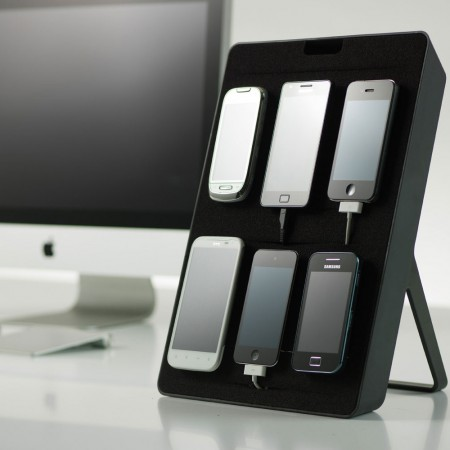
\includegraphics[width=9.1cm, height=6cm]{pwa/pwa-toolset-physical-devices/device-lab-stand}

Setting up ghost labs is as simple as running it in the mac application, and
being able to open on numerous devices. The following is a screenshot of what
you might see in your Ghostlab application:


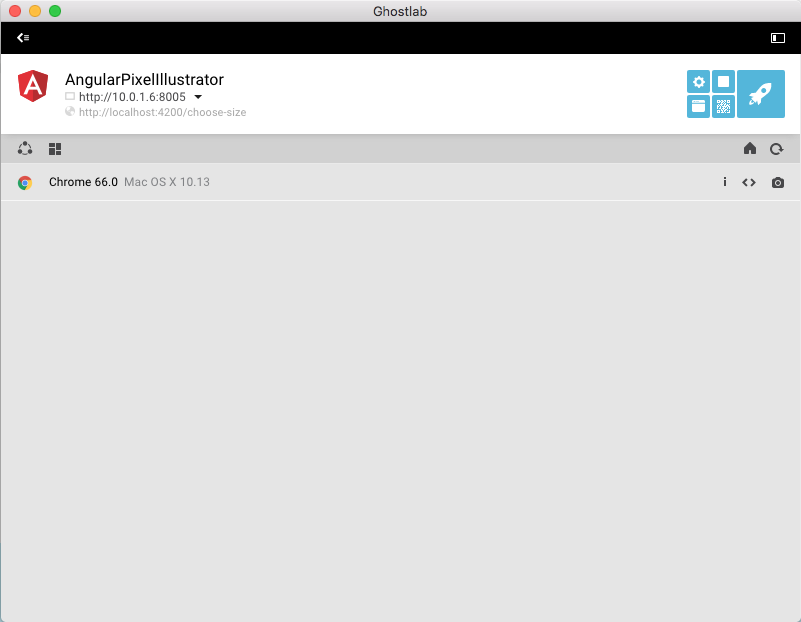
\includegraphics[width=9.1cm, height=6cm]{pwa/pwa-toolset-physical-devices/ghostlabs-screenshot}

Simply drag and drop the url of your browser into application. Click on the play
button. It will open up the above screenshot. You then have the option of
opening up the Ghost Labs generated url in any mobile device, by simply
scanning the qr code.

\subsection{ Notable Mentions of Ghost Labs }
\begin{enumerate}
  \item Synchronized browsing between different devices.
  \item Compile and refresh happens as if working with native CLI.
  \item Remote inspection of mobile devices.
  \item Remote screenshots.
\end{enumerate}

\subsection{ Final Words on Ghost Labs }
With regards to setting up responsive development workflow, Ghost Labs is next
to none. The \$49 dollar licensing fee is chump change. The amount of time
saved on infrastructure, is worth the investment. The device lab in addition
to buying actual current devices might go up to something in the ballpark of
\$1,000 to \$2,500.

However, this is arguably a fantastic decision. The engineers on your team have
8 hours a day to develop. Many times taken up by meetings, architectural
decisons, corporate events etc. Allowing them to seamlessly develop, without
having to re-configure their browser is a time saver. Perhaps somewhere around
1 hour a week. In addition, it helps promote developer happiness, by making
their life easier. At the end of the day, perhaps for this reason alone, it is
worth it.
